\documentclass{beamer}	% Compile at least twice!
%\setbeamertemplate{navigation symbols}{}
\usetheme{Warsaw}
%\useinnertheme{rectangles}
%\useoutertheme{infolines}
\useoutertheme[title,section,subsection=true]{smoothbars}
 
% -------------------
% Packages
% -------------------
\usepackage{
	amsmath,			% Math Environments
	amssymb,			% Extended Symbols
	enumerate,		    % Enumerate Environments
	graphicx,			% Include Images
	lastpage,			% Reference Lastpage
	multicol,			% Use Multi-columns
	multirow,			% Use Multi-rows
	pifont,			    % For Checkmarks
	stmaryrd,			% For brackets
}
\usepackage[french]{babel}
\usepackage[T1]{fontenc}


% -------------------
% Colors
% -------------------
\definecolor{UniOrange}{RGB}{212,69,0}
\definecolor{UniGray}{RGB}{62,61,60}
%\definecolor{UniRed}{HTML}{B31B1B}
%\definecolor{UniGray}{HTML}{222222}
\setbeamercolor{title}{fg=UniGray}
\setbeamercolor{frametitle}{fg=UniOrange}
\setbeamercolor{structure}{fg=UniOrange}
\setbeamercolor{section in head/foot}{bg=UniGray}
\setbeamercolor{author in head/foot}{bg=UniGray}
\setbeamercolor{date in head/foot}{fg=UniGray}
\setbeamercolor{structure}{fg=UniOrange}
\setbeamercolor{local structure}{fg=black}
\beamersetuncovermixins{\opaqueness<1>{0}}{\opaqueness<2->{15}}


% -------------------
% Fonts & Layout
% -------------------
\useinnertheme{default}
\usefonttheme{serif}
\usepackage{palatino}
\setbeamerfont{title like}{shape=\scshape}
\setbeamerfont{frametitle}{shape=\scshape}
\setbeamertemplate{itemize items}[circle]
%\setbeamertemplate{enumerate items}[default]


% -------------------
% Commands
% -------------------

% Special Characters
\newcommand{\N}{\mathbb{N}}
\newcommand{\Z}{\mathbb{Z}}
\newcommand{\Q}{\mathbb{Q}}
\newcommand{\R}{\mathbb{R}}
\newcommand{\C}{\mathbb{C}}

% Math Operators
\DeclareMathOperator{\im}{im}
\DeclareMathOperator{\Span}{span}

% Special Commands
\newcommand{\pf}{\noindent\emph{Proof. }}
\newcommand{\ds}{\displaystyle}
\newcommand{\defeq}{\stackrel{\text{def}}{=}}
\newcommand{\ov}[1]{\overline{#1}}
\newcommand{\ma}[1]{\stackrel{#1}{\longrightarrow}}
\newcommand{\twomatrix}[4]{\begin{pmatrix} #1 & #2 \\ #3 & #4 \end{pmatrix}}

% -------------------
% Tikz & PGF
% -------------------
\usepackage{tikz}
\usepackage{tikz-cd}
\usetikzlibrary{
	calc,
	decorations.pathmorphing,
	matrix,arrows,
	positioning,
	shapes.geometric,
	automata, 
	chains, 
	arrows.meta, quotes
}
\usepackage{pgfplots}
\pgfplotsset{compat=newest}


% -------------------
% Theorem Environments
% -------------------
\theoremstyle{plain}
\newtheorem{thme}{Théorèm}[section]
\newtheorem{policy}{Policy Evaluation}[section]
\newtheorem{obj}{Objectif}[section]
\newtheorem{prop}{Proposition}[section]
\newtheorem{lem}{Lemma}[section]
\newtheorem{cor}{Corollary}[section]
\theoremstyle{definition}
\newtheorem{concl}{Conclusion}[section]

\newtheorem{eq}{Equation}[section]
\newtheorem{ex}{Example}[section]

\newtheorem{dfn}{Definition}[section]
\theoremstyle{remark}
\newtheorem{rem}{Remark}[section] 
\numberwithin{equation}{section}



% -------------------
% Title Page
% -------------------
\title{\textcolor{white}{Sutton Barto Learning}}
\subtitle{\textcolor{white}{Chaptre 6: Temporal Difference Learning}}  
\author{\\ Elkael \bsc{MAXIME}\\Bin \bsc{LIU} }
\date{Master2 Informatique AMIS Paris Saclay \\UVSQ 2019-2020}



% -------------------
% Content
% -------------------
\begin{document}


% Title Page
\begin{frame}
\titlepage
\end{frame}



% Sommaire
\section{Sommaire}

% Mon Sommaire
\begin{frame}

\begin{block}{Sommaire :}
\begin{itemize}
	\item Méthode TD(0)
	\item Présentation du jeu du taxi
	\item Sarsa: On-Policy control.
	\item Q-learning: Off-Policy control
\end{itemize}
\end{block}
	
\end{frame}

% Métohde TD (0) 
\section{Métohde TD (0) }

% Definitions & Examples
\begin{frame}
Equation de Bellman pour TD(0) (vue en cours):
\begin{eq}
\begin{equation}
    V(S_{t}) \leftarrow V(S_{t}) + \alpha \left [ R_{t+1} + V(S_{t+1}) - V(S_{t}) \right ] ;
\end{equation}
    $\alpha \in \left [ 0,1 \right ]$ : le facteur d'apprentissage;
\end{eq}
\end{frame}

\begin{frame}
Equation de Bellman pour TD(0) avec discount:
\begin{eq}

\begin{equation}
    V(S_{t}) \leftarrow V(S_{t}) + \alpha \left [ R_{t+1} + \gamma V(S_{t+1}) - V(S_{t}) \right ] ;
\end{equation}
    $\alpha \in \left [ 0,1 \right ]$ : le facteur d'apprentissage
    \\
    $\gamma \in \left [ 0,1 \right ]$ : le facteur de réduction
    \\
\end{eq}
Les récompenses les plus lointaines dans le temps ont une probabilité plus faible d'arriver.
\end{frame}

\begin{frame}

Rappel sur l'éxecution de TD(0):
\begin{ex}
\begin{center}
\begin{tikzpicture}[auto,node distance = 10mm,start chain = going right,state/.append style = {thick,  minimum width=1.5em,text width=1.5em,align=center,on chain,fill=white,text=black
 },
]

\node (s0)[state]    {$A$};   
\node (s1)[state]    {$B$};  
\node (s2)[state]    {$C$};  

\draw[->] (s0) edge[bend left] node (a1) {$R_{A}$} (s1)
          (s0) edge[bend right] node (b1) {$R_{A}^{'}$} (s1)
          (s1) edge[bend left] node (a2) {$R_{B}$} (s2)
          (s1) edge[bend right] node (b2) {$R_{B}^{'}$} (s2);
\end{tikzpicture}
\\
$V(A)$ = $V(B)$ = $V(C)$ = 0 au début de l'estimation
\end{center}

\begin{figure}
\begin{minipage}[t]{1\linewidth}
\centering
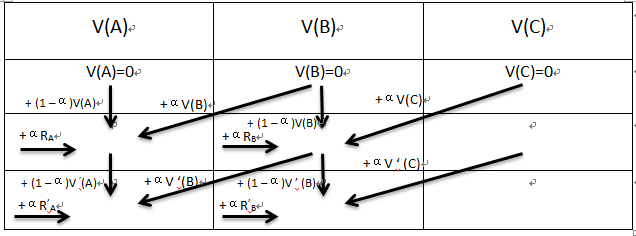
\includegraphics[width=0.90 \textwidth,height=0.5\textheight]{photo/ex.png}
\label{fig:side:a}
\end{minipage}%

\end{figure}
\end{ex}
\end{frame}


\begin{frame}
Les récompenses les plus lointaines dans le temps ont une probabilité plus faible d'arriver.
\begin{eq}

\begin{equation}
    V(S_{t}) \leftarrow V(S_{t}) + \alpha \left [ R_{t+1} + \gamma V(S_{t+1}) - V(S_{t}) \right ] ;
\end{equation}
    Gain: $G_{t} = R_{t} + \gamma R_{t+1} + ... + \gamma^n R_{t+n}$
    \\
    $ V(S_{t}) = E[G_{t}]$
\end{eq}
\end{frame}



\iffalse
% MC Méthode
\section{Monte Carlo Méthode}

% MC 
\begin{frame}
Monte Carlo Méthode:

\begin{eq}
On a l'équation suivante (on attend la fin de plusieurs récompenses avant d'estimer la valeur de la stratégie) :

\begin{equation}
    V(S_{t}) \leftarrow V(S_{t}) + \alpha \left [ G(S_{t}) - V(S_{t}) \right ] ;
\end{equation}
Le somme de tous les récompenses:
\begin{equation}
    G_{t}= R_{t} + \gamma R_{t+1} + ... + \gamma_{n} R_{t+n};
\end{equation}
\end{eq}
\end{frame}
\fi

% Application 1
\begin{frame}
    \begin{figure}[h!]
    \centering
    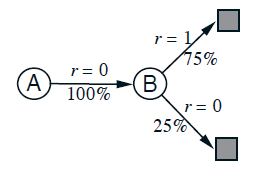
\includegraphics[width=0.60 \textwidth,height=0.35\textheight]{photo/img.png}
    \caption{Le modèle de chaîne de markov}
    \label{fig:graphe1}
    \end{figure}

On considère 8 épisodes : 
	
	B; 1        \qquad \qquad A; 0; B; 0   \\
	B; 1        \qquad \qquad B; 1  \\
	B; 1        \qquad \qquad  B; 1  \\
	B; 1        \qquad \qquad B; 1  \\
	B; 1        \qquad \qquad B; 0  \\

\end{frame}



% Math
\begin{frame}
Pour B, $V(B) = 3/4 $ , une seule solution! 

Pour A, 2 choix possibles : 
\begin{itemize}
	\item Méthode de Monte Carlo: $V(A) = 0 $  en moyenne.
	\item Méthode TD(0): $V(A) = 3/4 $ car A mène toujours à B.
\end{itemize} 

Intuition: 
\begin{itemize}
	\item TD (0): le résultat correspond au modèle qui a le plus probablement généré ces données.
	\item Monte Carlo: le résultat correspond exactement aux données.
\end{itemize} \vspace{0.5cm}

\begin{policy}
Dans un jeu à 1 joueur, en fixant la stratégie $\pi$, on se ramène à un jeu à 0 joueur et on peut appliquer TD(0) pour évaluer cette stratégie
\end{policy}
\end{frame}

\begin{frame}
Un exemple d'éxecution dans un jeu à 1 joueur : le jeu du taxi
\begin{figure}
\begin{minipage}[t]{0.5\linewidth}
\centering
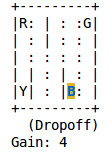
\includegraphics[width=0.60 \textwidth,height=0.35\textheight]{photo/jeux.png}
\label{fig:side:a}
\end{minipage}%
\end{figure}
\begin{itemize}

\item 500 états (grille 5 * 5, 5 positions possibles pour le passager, 4 destinations possibles)
\item 6 actions : haut, bas, gauche, droite, pickup, drop-off.
\item Récompenses : -1 par tour de jeu, +20 pour déposer le passager, -10 pour pickup/dropoff illégal.
\item Jeu fini: dans tous les cas au bout de 200 étapes on stoppe le jeu
\end{itemize}
\end{frame}


\begin{frame}

Q-learning et SARSA : trouver une stratégie optimale dans les jeux à 1 joueur à horizon fini

\end{frame}

\begin{frame}

\begin{ex}
\centering
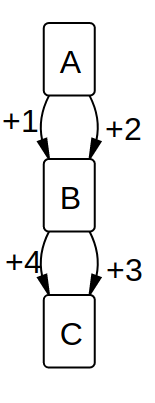
\includegraphics[width=0.30
\textwidth,height=0.6\textheight]{photo/1joueurV.png}
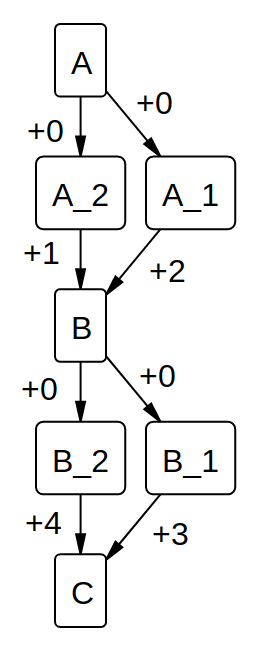
\includegraphics[width=0.30
\textwidth,height=0.6\textheight]{photo/1joueur.png}
\end{ex}
\end{frame}

\begin{frame}

\begin{itemize}
    \item On définit la fonction Q(S, A) comme la fonction qui donne la valeur d'une action A dans l'état S
    \item La stratégie optimale est la stratégie qui maximise toutes les Q values pour toutes les actions qu'elle choisit
    \item Donc on cherche à calculer Q pour tous les couples (S, A) pour en déduire la stratégie optimale
\end{itemize}

\end{frame}

\begin{frame}

\begin{itemize}
    \item On cherche à améliorer la stratégie qu'on a déja découverte (exploitation) donc on va jouer les actions qui ont la meilleure Q-value (stratégie gloutonne)
    \item Si on joue uniquement nos meilleures actions on rate peut etre des opportunités d'innover pour s'améliorer
\end{itemize}
\begin{itemize}
    \item Pour aider l'exploration on joue donc une stratégie $\epsilon$-gloutonne, c'est à dire qu'on joue aléatoirement avec proba $\epsilon$
\end{itemize}

\end{frame}


% Sarsa
\section{Sarsa}

\begin{frame}

Sarsa: Choisir une stratégie optimale dans un jeu à un joueur

\begin{figure}
\begin{minipage}[t]{1\linewidth}
\centering
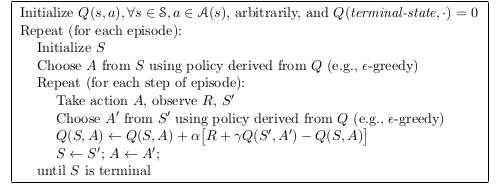
\includegraphics[width=0.80 \textwidth,height=0.6\textheight]{photo/sarsa.png}
\label{fig:side:a}
\end{minipage}%

\end{figure}
\end{frame}



% Q-learning
\section{Q-learning}
\begin{frame}

Q-learning: Choisir une stratégie optimale dans un jeu à un joueur

\begin{figure}
\begin{minipage}[t]{1\linewidth}
\centering
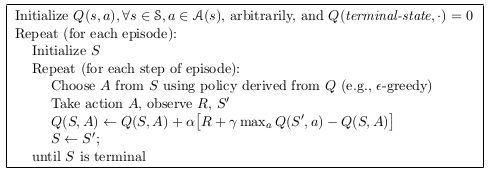
\includegraphics[width=0.80 \textwidth,height=0.6\textheight]{photo/Q.png}
\label{fig:side:a}
\end{minipage}%

\end{figure}
\end{frame}


% Jeux
\section{Pratique sur le jeux}

\begin{frame}
Sarsa: on-policy, Q-learning: off-policy
\begin{itemize}
\item Sarsa :
$Q(S_t, A_t) \leftarrow Q(S_t, A_t) + \alpha[R_{t+1} + \gamma Q(S_{t+1}, A_{t+1})-Q(S_t, A_t)]$
\end{itemize}

\vspace{0.5cm}

\begin{itemize}
\item Q-learning :
$Q(S_t, A_t) \leftarrow Q(S_t, A_t) + \alpha[R_{t+1} + \gamma max_a Q(S_{t+1}, a)-Q(S_t, A_t)]$
\end{itemize}

\vspace{1.0cm}


La mise à jour donnée par Q-learning ne dépend pas de l'action effectuée, donc Q-learning peut apprendre la stratégie optimale sans suivre la stratégie qu'il est en train d'apprendre.
\end{frame}


% Conclusion
\section{Conclusion}
% End Slide
\begin{frame}
\begin{concl}
Limites de ces algos:
\begin{itemize}
    \item Si l'espace d'états/actions est très grand: peu réaliste
    \item Si l'espace d'actions ou d'états est continu, on ne peut pas directement représenter le jeu par un tableau
    
\end{itemize}
\end{concl}
\end{frame}


% Questions
\begin{frame}
\begin{center} {\bfseries \Large Questions?} \end{center}
\end{frame}



\end{document}